\documentclass[11pt,a4paper]{article}

\usepackage[utf8]{inputenc}
\usepackage[T1]{fontenc}
\usepackage[margin=2.5cm]{geometry}
\usepackage{graphicx}
\usepackage{booktabs}
\usepackage{longtable}
\usepackage{array}
\usepackage{amsmath,amssymb}
\usepackage{xcolor}
\usepackage{listings}
\usepackage{float}
\usepackage{subcaption}
\usepackage{tikz}
\usetikzlibrary{shapes.geometric, arrows.meta, positioning, fit, backgrounds}
\usepackage[numbers,sort&compress]{natbib}
\usepackage[colorlinks=true,linkcolor=blue!60!black,citecolor=blue!60!black,urlcolor=blue!60!black]{hyperref}
\usepackage[nameinlink,noabbrev]{cleveref}

\graphicspath{{figures/}}

\lstset{
    basicstyle=\ttfamily\small,
    breaklines=true,
    frame=single,
    backgroundcolor=\color{gray!6},
    rulecolor=\color{gray!35},
    xleftmargin=0.5em,
    xrightmargin=0.5em,
    columns=flexible
}

\title{%
    \textbf{LLM-Assisted Evidence Extraction for 4--20mer Peptide Self-Assembly Literature}\\[0.5em]
    \large Technical Report Draft
}

\author{%
    Can Ersoy\\
    \texttt{can.ersoy@tum.de}
}

\date{\today}

\begin{document}

\maketitle

\begin{abstract}
Experimental records on short-peptide self-assembly---encompassing primary amino acid sequences, terminal modifications, solvent systems, reaction conditions, nanostructure morphologies, and characterization techniques---are dispersed across tens of thousands of scientific publications. Existing curated resources such as SAPdb, CPAD~2.0, WaltzDB~2.0, and Cross-Beta~DB are fragmented, cover narrow sequence or morphology scopes, and rely on manual curation that does not scale. We present \texttt{peptide\_extractor}, an end-to-end automated literature curation pipeline targeting 4--20mer peptide self-assembly. The system integrates multi-provider literature discovery (NCBI PubMed/PMC, Scopus, OpenAlex, Semantic Scholar), high-recall abstract-level relevance screening via Large Language Models (LLMs), full-text retrieval backed by Azure Blob Storage, unified structural parsing of JATS~XML, GROBID TEI~XML, and scholarly PDFs into a citation-grounded node tree, and schema-constrained multimodal LLM extraction. To support both large-scale deployment without ground truth and rigorous quantitative validation, we combine reference-free completeness and citation-grounding verification with normalized matching against a manually curated golden benchmark. Across a 10-paper multi-table development benchmark, transitioning from text-only single-pass extraction to direct PDF and multimodal table-image extraction raised sequence F1 from $40.5\%$ to $92.0\%$ and condition row recall from $3.2\%$ ($17/530$) to $70.0\%$ ($371/530$).
\end{abstract}

\tableofcontents
\newpage

\section{Introduction}
\label{sec:introduction}

Short-peptide self-assembly is a foundational mechanism in supramolecular biomaterials, nanomedicine, and amyloid pathology. Oligopeptides spanning roughly 4 to 20 amino acid residues---together with shorter capped di- and tri-peptide motifs such as Fmoc-Phe-Phe---spontaneously organize into diverse nanostructures including hydrogels, nanofibers, nanotubes, nanospheres, ribbons, vesicles, and cross-$\beta$ amyloid fibrils. Whether a given sequence assembles, and which morphology it adopts, depends sensitively on experimental parameters: terminal modifications ($N$- and $C$-terminal caps), peptide concentration, solvent and co-solvent ratios, pH, temperature, incubation time, and sample preparation protocols.

Despite decades of experimental publications, this knowledge remains fragmented across tens of thousands of unstructured journal articles, tables, figure captions, and supplementary documents. Existing manually curated repositories---such as SAPdb~\cite{sapdb2020}, WALTZ-DB~2.0~\cite{waltzdb2020}, CPAD~2.0~\cite{cpad2020}, and Cross-Beta~DB~\cite{crossbetadb2024}---each cover restricted sequence lengths, specific morphological subsets, or incompatible schemas, and manual curation cannot keep pace with new literature.

Automating the extraction of experimental peptide self-assembly records using Large Language Models (LLMs) presents four core technical challenges:
\begin{enumerate}
    \item \textbf{Literature Triage at Scale:} Broad bibliographic queries return tens of thousands of candidate papers, many of which are reviews, purely computational studies, or investigations of full-length proteins rather than isolated short peptides. Downloading and processing full texts for all candidates is wasteful in bandwidth, storage, and LLM token cost.
    \item \textbf{Heterogeneous Document Formats:} Open-access articles may be available as structured JATS~XML (e.g., PubMed Central) or only as scholarly PDFs, where dense multi-column screening tables and characterization figures carry critical experimental matrices.
    \item \textbf{Matrix Unrolling and Paper-Wide Defaults:} A single publication frequently reports dozens of peptides across multiple solvent or pH conditions in compact tables while stating shared parameters (e.g., temperature, buffer, detection methods, preparation protocol) once in the Methods prose. Single-pass text-only LLM prompts routinely truncate large tables or drop paper-wide defaults.
    \item \textbf{Auditability and Grounding:} Extracted records must not rely on unverified model generations; every claimed field should be traceable back to an exact sentence, table, or figure in the source publication, and extraction quality must be measurable even when no ground-truth annotations exist.
\end{enumerate}

To address these challenges, we developed \texttt{peptide\_extractor}, an end-to-end literature curation pipeline for 4--20mer peptide self-assembly research. The system combines multi-provider bibliographic retrieval, high-recall abstract relevance screening, unified JATS~XML / TEI~XML / PDF parsing into a citation-grounded node tree, multimodal and two-pass factored LLM extraction, and dual evaluation via reference-free grounding checks and normalized golden-dataset benchmarking.

\section{Background and Data Schema}
\label{sec:background}

\subsection{Existing Peptide Self-Assembly Databases}
Several domain databases catalog experimentally characterized self-assembling or amyloidogenic peptides, each with distinct scope and curation methodology:
\begin{itemize}
    \item \textbf{SAPdb}~\cite{sapdb2020}: Collates 1,049 entries from 301 research articles on self-assembling di- and tri-peptides forming discrete nanostructures (nanotubes, nanofibers, hydrogels, nanospheres, nanovesicles), capturing terminal modifications, solvent, concentration, pH, temperature, incubation time, and morphology.
    \item \textbf{WALTZ-DB~2.0}~\cite{waltzdb2020}: Focuses on amyloid-forming hexapeptides across curated subsets (e.g., FUS, TDP-43, SOD-1, Sup35, functional amyloids, and literature-mined hexapeptides).
    \item \textbf{CPAD~2.0}~\cite{cpad2020}: Aggregates experimental data on aggregating proteins and peptides, incorporating entries from WALTZ-DB and AmyPro alongside aggregation kinetics.
    \item \textbf{Cross-Beta~DB}~\cite{crossbetadb2024}: Catalogs 272 experimentally determined 3D cross-$\beta$ amyloid fibril structures selected from the Protein Data Bank (PDB).
    \item \textbf{AmyPro, AmyloGraph, and AmyloBase}: Specialized resources covering amyloidogenic regions, aggregation modulators, and kinetic curves.
\end{itemize}
While these resources provide valuable ground truth, they are siloed, use inconsistent field definitions (e.g., mixed concentration units, unstandardized terminal cap labels, or placeholder strings such as \texttt{NP}), and omit most 4--20mer non-amyloid nanostructure literature.

\subsection{Golden Benchmark Construction}
To benchmark automated extraction, we consolidated entries from SAPdb, PeptideMiner, CPAD~2.0, and Cross-Beta~DB into a unified golden dataset (\texttt{golden\_dataset\_final.csv}) and ingested manually curated ground-truth records into the pipeline database under \texttt{ExtractionMode.MANUAL} (\texttt{run\_identifier=0}). For SAPdb and PeptideMiner golden papers, 71 of 75 target publications were successfully acquired (13 already present in the database via open-access full text and 58 manually downloaded PDFs uploaded to Azure Blob Storage). Within this corpus, a 10-paper development slice (\texttt{DEV\_BENCHMARK\_PMIDS}) containing 56 unique peptide sequences and 530 experimental condition rows (253 assembling, 277 non-assembling) serves as a rapid-iteration benchmark covering challenging multi-table matrices, cyclic peptides, peptide mixtures, and varied terminal notations.

\subsection{Standardized \texttt{PeptideEntry} Schema}
Each extracted or manually curated record is stored as a \texttt{PeptideEntry} row in SQLite via SQLModel. \Cref{tab:peptide_schema} summarizes the core fields, types, and conventions. Missing or unstated experimental parameters are stored as \texttt{NULL} rather than legacy placeholders.

\begin{table}[htbp]
\centering
\caption{Core fields of the standardized \texttt{PeptideEntry} schema.}
\label{tab:peptide_schema}
\small
\begin{tabular}{@{}llp{7.8cm}@{}}
\toprule
\textbf{Field} & \textbf{Type} & \textbf{Description and Canonical Conventions} \\
\midrule
\texttt{sequence} & String & Uppercase single-letter IUPAC amino acid sequence (e.g., \texttt{FF}, \texttt{KLVFF}, \texttt{VQIVYK}). \\
\texttt{length} & Integer & Residue count computed from \texttt{sequence} (target: 4--20mer; benchmark includes 2--43). \\
\texttt{type} & Enum & Morphological outcome: \texttt{hydrogel}, \texttt{fiber}, \texttt{tube}, \texttt{nanosphere}, \texttt{ribbon}, \texttt{vesicle}, \texttt{particle}, \texttt{organogel}, \texttt{amyloid}, or \texttt{none}. \\
\texttt{n\_terminal} / \texttt{c\_terminal} & String & Terminal modifications (e.g., \texttt{Fmoc}, \texttt{Acetylation}, \texttt{Amidation}, \texttt{Free}). \\
\texttt{linear\_cyclic} & String & Backbone topology: \texttt{linear} or \texttt{cyclic}. \\
\texttt{chirality} & String & Stereochemistry: \texttt{L}, \texttt{D}, \texttt{heterochiral}, \texttt{racemic}, or \texttt{achiral}. \\
\texttt{peptide\_conjugate\_mixture} & String & System class: \texttt{peptide}, \texttt{conjugate}, or \texttt{mixture}, plus optional \texttt{conjugate\_partner}. \\
\texttt{temperature} & Float & Reaction temperature in $^\circ$C (room temperature normalized to $25.0\,^\circ\text{C}$). \\
\texttt{ph} & Float & Solution pH. \\
\texttt{peptide\_concentration} & Float & Concentration normalized to $\text{mg/ml}$ (e.g., $1\,\text{wt\%} \rightarrow 10.0\,\text{mg/ml}$). \\
\texttt{solution} / \texttt{solvent} & String & Primary dispersion medium/buffer and organic co-solvent (e.g., \texttt{PBS}, \texttt{DMSO}). \\
\texttt{volume\_ratio} & String & Mixing ratio ($v/v$), formatted as \texttt{"5/95"} or \texttt{"1"} for neat systems. \\
\texttt{incubation\_period} & Integer & Incubation duration normalized to minutes. \\
\texttt{detection\_method} & String & Comma-separated characterization techniques (e.g., \texttt{TEM}, \texttt{Cryo-EM}, \texttt{ThT}, \texttt{CD}). \\
\texttt{preparation\_protocol} & Text & Verbatim sample preparation and dissolution protocol from the paper. \\
\texttt{evidence\_span} & JSON & Maps 12 extracted fields to bracketed node location tags (e.g., \texttt{[sec-1/table-0]}). \\
\texttt{paper\_id} & Integer & Foreign key linking to \texttt{paper\_metadata.id}. \\
\bottomrule
\end{tabular}
\end{table}

\section{System Architecture}
\label{sec:architecture}

\texttt{peptide\_extractor} is implemented as a modular Python package (\texttt{src/peptide\_extractor/}) orchestrated by \texttt{pipeline.py} and exposed through a YAML-configurable Click CLI (\texttt{cli.py}). All metadata, screening decisions, extraction records, and evaluation metrics reside in a central SQLite database managed via SQLModel and Alembic migrations, while large full-text payloads (JATS~XML and PDFs) are stored in Azure Blob Storage with local filesystem caching.

\Cref{fig:pipeline_arch} illustrates the five logical stages of the end-to-end pipeline.

\begin{figure}[htbp]
\centering
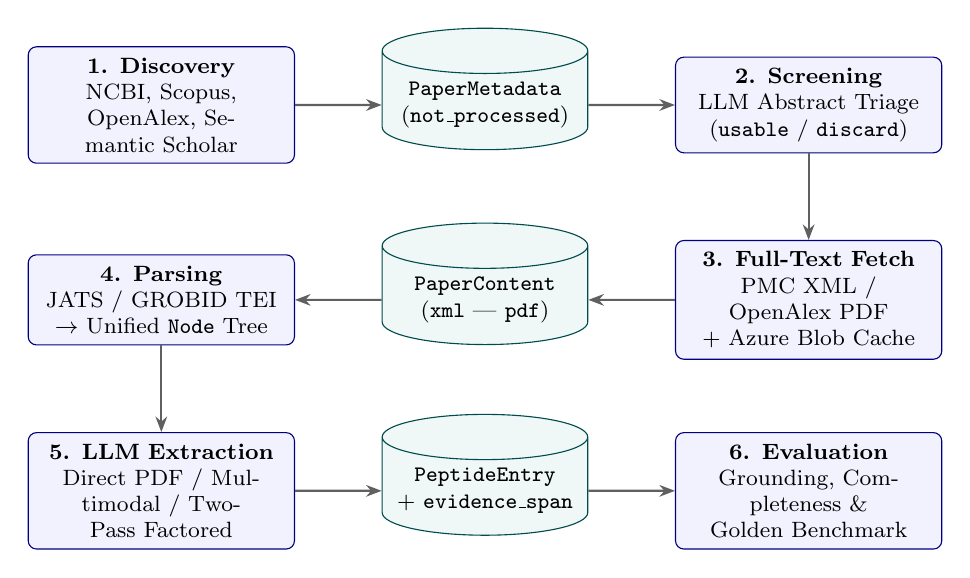
\begin{tikzpicture}[
    node distance=0.85cm and 1.1cm,
    box/.style={rectangle, rounded corners=3pt, draw=blue!50!black, fill=blue!5, text width=3.1cm, align=center, font=\footnotesize, minimum height=0.95cm, inner sep=4pt},
    db/.style={cylinder, shape border rotate=90, draw=teal!60!black, fill=teal!6, aspect=0.22, text width=2.4cm, align=center, font=\footnotesize, minimum height=0.85cm, inner sep=3pt},
    arrow/.style={-{Stealth[scale=0.85]}, thick, draw=gray!75!black}
]
    \node[box] (s1) {\textbf{1. Discovery}\\NCBI, Scopus, OpenAlex, Semantic Scholar};
    \node[db, right=of s1] (pm) {\texttt{PaperMetadata}\\(\texttt{not\_processed})};
    \node[box, right=of pm] (s2) {\textbf{2. Screening}\\LLM Abstract Triage\\(\texttt{usable} / \texttt{discard})};

    \node[box, below=1.1cm of s2] (s3) {\textbf{3. Full-Text Fetch}\\PMC XML / OpenAlex PDF\\+ Azure Blob Cache};
    \node[db, left=of s3] (pc) {\texttt{PaperContent}\\(\texttt{xml} | \texttt{pdf})};
    \node[box, left=of pc] (s4) {\textbf{4. Parsing}\\JATS / GROBID TEI\\$\rightarrow$ Unified \texttt{Node} Tree};

    \node[box, below=1.1cm of s4] (s5) {\textbf{5. LLM Extraction}\\Direct PDF / Multimodal / Two-Pass Factored};
    \node[db, right=of s5] (pe) {\texttt{PeptideEntry}\\+ \texttt{evidence\_span}};
    \node[box, right=of pe] (s6) {\textbf{6. Evaluation}\\Grounding, Completeness \& Golden Benchmark};

    \draw[arrow] (s1) -- (pm);
    \draw[arrow] (pm) -- (s2);
    \draw[arrow] (s2) -- (s3);
    \draw[arrow] (s3) -- (pc);
    \draw[arrow] (pc) -- (s4);
    \draw[arrow] (s4) -- (s5);
    \draw[arrow] (s5) -- (pe);
    \draw[arrow] (pe) -- (s6);
\end{tikzpicture}
\caption{End-to-end \texttt{peptide\_extractor} pipeline architecture from literature discovery to evaluation.}
\label{fig:pipeline_arch}
\end{figure}

\subsection{Relational Data Models and Lifecycles}
Six SQLModel tables track provenance across every stage:
\begin{itemize}
    \item \texttt{raw\_provider\_record} (\texttt{RawProviderRecord}): Archives raw provider search payloads prior to normalization.
    \item \texttt{paper\_metadata} (\texttt{PaperMetadata}): Canonical paper record (\texttt{doi}, \texttt{pmid}, \texttt{pmcid}, \texttt{title}, \texttt{abstract}, \texttt{status}, \texttt{dataset\_subset}, \texttt{source\_databases}). Papers transition through \texttt{PaperStatus}: \texttt{not\_processed} $\rightarrow$ \texttt{usable} or \texttt{discard}, and are tagged as \texttt{golden\_benchmark} or \texttt{scraped} via \texttt{DatasetSubset}.
    \item \texttt{paper\_relevance} (\texttt{PaperRelevance}): Stores abstract screening verdicts (\texttt{is\_relevant}, \texttt{confidence}, \texttt{detected\_clues}, \texttt{explanation}), model identifier, and \texttt{run\_identifier}.
    \item \texttt{paper\_content} (\texttt{PaperContent}): Links each paper to its full-text artifact (\texttt{format} $\in \{\texttt{xml}, \texttt{pdf}\}$, \texttt{blob\_url}, \texttt{pdf\_url}, \texttt{source}).
    \item \texttt{peptide\_entry} (\texttt{PeptideEntry}): Stores extracted or manual peptide records (\texttt{ExtractionMode.LLM} vs.\ \texttt{ExtractionMode.MANUAL}).
    \item \texttt{extraction\_evaluation} (\texttt{ExtractionEvaluation}): Persists reference-free \texttt{completeness\_rate}, \texttt{groundness\_rate}, and \texttt{faithfulness\_rate} per \texttt{PeptideEntry}.
\end{itemize}

\subsection{CLI Execution and Observability}
The CLI exposes \texttt{run\_pipeline --config config.yaml}, which executes configurable sequences of steps (\texttt{search}, \texttt{deduplicate}, \texttt{find\_abstracts}, \texttt{clean\_empty}, \texttt{relevance}, \texttt{fetch\_fulltext}, \texttt{extraction}, \texttt{evaluation}, \texttt{visualization}), each tagged with a \texttt{run\_identifier} and routed to per-step log files (\texttt{docs/logs/[step]/\{run\_identifier\}.log}). A standalone \texttt{visualize} command exports publication-ready PNG/SVG charts across all database tables via \texttt{visualization.py}.

\section{Literature Retrieval and Abstract Screening}
\label{sec:retrieval_screening}

\subsection{Multi-Provider Retrieval and Metadata Cleaning}
Literature discovery (\texttt{providers.py}) queries multiple bibliographic APIs using structured boolean queries pairing oligopeptide length terms (\texttt{tetrapeptide} through \texttt{eicosapeptide}/\texttt{icosapeptide}) with self-assembly morphology keywords (\texttt{nanostructure}, \texttt{nanotube}, \texttt{nanofiber}, \texttt{nanorod}, \texttt{hydrogel}, \texttt{nanosphere}, \texttt{nanoparticle}, \texttt{self-assembly}), filtered to English primary research articles where supported:
\begin{itemize}
    \item \textbf{NCBIProvider}: Queries PubMed and PubMed Central (PMC) via E-Utilities (\texttt{esearch}/\texttt{efetch}) with API key authentication, batching (100--150 IDs per request), and rate-limit delays.
    \item \textbf{ScopusProvider}: Queries the Elsevier Scopus Search API for title/abstract/keyword metadata.
    \item \textbf{OpenAlexProvider} and \textbf{SemanticScholarProvider}: Provide auxiliary metadata, DOI-based abstract backfilling (\texttt{find\_abstracts\_by\_doi}), and Open Access PDF URL discovery.
\end{itemize}
Following ingestion, \texttt{deduplicate\_by\_doi()} normalizes DOIs and removes duplicate records, \texttt{find\_abstracts\_by\_doi()} backfills missing abstracts via OpenAlex, and \texttt{remove\_empty\_abstract\_title\_papers()} prunes entries lacking usable metadata. For papers marked \texttt{PaperStatus.USABLE}, \texttt{fetch\_paper\_fulltexts()} retrieves PMC JATS~XML first and falls back to OpenAlex PDFs, storing payloads in Azure Blob Storage (\texttt{azure\_storage.py}) with local caching.

\subsection{Stage 1: High-Recall Abstract Relevance Screening}
Before downloading full texts, \texttt{relevance.py} triages \texttt{not\_processed} papers using only their title and abstract. Screening supports both single-paper mode (\texttt{screen\_papers}) and batched bulk mode (\texttt{bulk\_screen\_papers}, default \texttt{batch\_size=50}), returning structured \texttt{RelevanceResult} objects containing \texttt{detected\_clues}, \texttt{explanation}, \texttt{is\_relevant}, and \texttt{confidence} $\in [0.0, 1.0]$.

The system prompt explicitly prioritizes \textbf{high recall}: borderline wet-lab papers are retained as relevant (with lower confidence), and only unambiguously out-of-scope studies---purely computational/theoretical papers without experimental validation, review articles, or studies exclusively on intact full-length proteins---are discarded.

\begin{table}[htbp]
\centering
\caption{Abstract screening recall on 1,000 sampled papers across LLM backends.}
\label{tab:relevance_recall}
\begin{tabular}{@{}lcc@{}}
\toprule
\textbf{Model} & \textbf{Recall} & \textbf{Run Identifier} \\
\midrule
Llama 3.2 3B & 0.970 & \texttt{1794483970} \\
Gemini 3.5 Flash Lite & 0.886 & \texttt{1794437084} \\
Gemini 3.1 Flash Lite & 0.873 & \texttt{1794437892} \\
DeepSeek R1 8B & 0.816 & \texttt{1794491078} \\
\bottomrule
\end{tabular}
\end{table}

On a 119-paper golden benchmark subset, Gemini~3.5~Flash~Lite and Gemma~31B each retained 118/119 papers, while Llama~3.2~3B retained 115/119. Across a 1,000-paper recall sample (\Cref{tab:relevance_recall}), Llama~3.2~3B achieved the highest recall ($0.970$) at zero API cost via local Ollama inference, making it suitable for large-scale pre-filtering. Applied to the full $\sim$50,020-paper scraped corpus, Llama~3.2~3B classified 28,664 papers as relevant and filtered out 21,356 non-relevant papers ($42.7\%$ reduction in downstream full-text processing). \Cref{fig:relevance_conf} compares confidence score distributions between Gemini and Llama~3.2~3B on large screening runs.

\begin{figure}[htbp]
\centering
\begin{subfigure}[b]{0.48\textwidth}
    \centering
    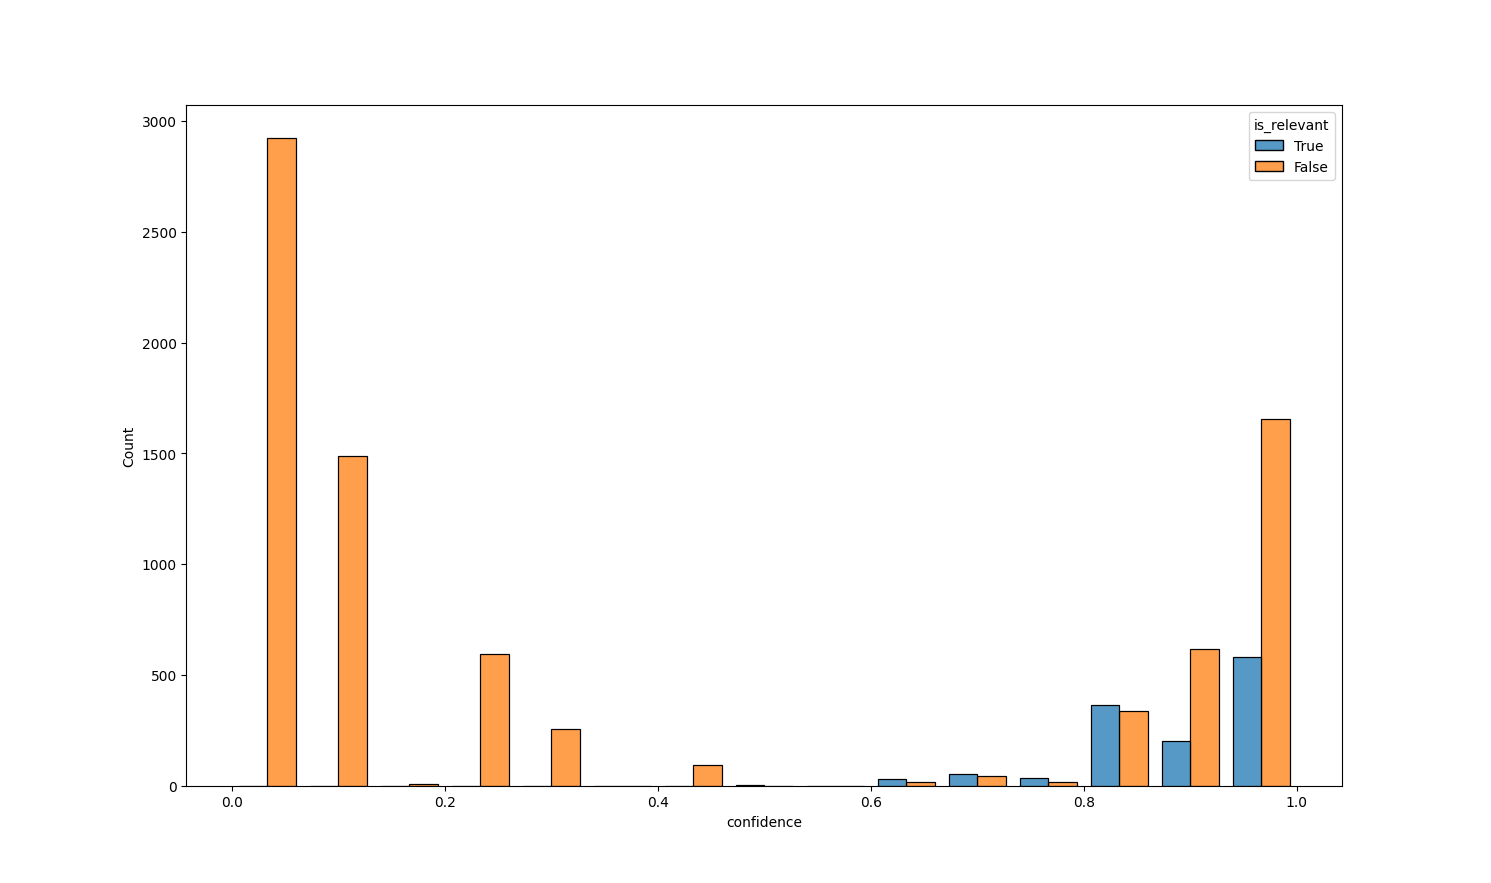
\includegraphics[width=\textwidth]{confidence-gemini-10k.png}
    \caption{Gemini (10k-paper run)}
    \label{fig:conf_gemini}
\end{subfigure}
\hfill
\begin{subfigure}[b]{0.48\textwidth}
    \centering
    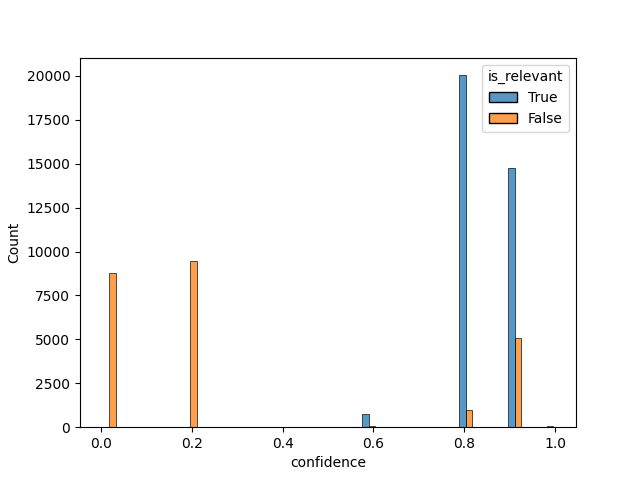
\includegraphics[width=\textwidth]{confidence-llama-complete.png}
    \caption{Llama 3.2 3B (full corpus)}
    \label{fig:conf_llama}
\end{subfigure}
\caption{Abstract relevance screening confidence distributions across models.}
\label{fig:relevance_conf}
\end{figure}

\section{Unified Document Parsing and Citation Grounding}
\label{sec:parsing}

Scientific full texts arrive in heterogeneous formats: structured JATS~XML from PubMed Central or scholarly PDFs from OpenAlex and manual curation. To ensure downstream extraction prompts and grounding evaluators operate identically across formats, \texttt{parsers.py} and \texttt{table\_renderer.py} convert all documents into a unified, citation-grounded \texttt{Node} object tree.

\subsection{Format Auto-Detection and GROBID Conversion}
\texttt{parse\_document(content, format="auto", ...)} automatically dispatches input payloads:
\begin{enumerate}
    \item \textbf{PDF Input:} Detected via \texttt{\%PDF} magic bytes or \texttt{.pdf} suffix. \texttt{GrobidClient} submits the PDF to a GROBID~\cite{grobid} REST service (\texttt{/api/processFulltextDocument}) to produce TEI~XML. When table or figure cropping is enabled, \texttt{tei\_coordinates=["figure"]} is requested so every table and figure carries PDF page bounding boxes (\texttt{coords}).
    \item \textbf{TEI~XML Input:} Detected via \texttt{<TEI}, \texttt{<teiHeader}, or the TEI namespace.
    \item \textbf{JATS~XML Input:} Default XML fallback for PMC full-text articles.
\end{enumerate}

\subsection{Hierarchical \texttt{Node} Tree and Sentence Segmentation}
\texttt{parse\_xml()} traverses the \texttt{<body>} (or \texttt{<text>}) element using \texttt{BeautifulSoup(..., "xml")}, naturally excluding reference lists (\texttt{<ref-list>}), acknowledgments, and boilerplate to preserve LLM context budget. Every element receives a deterministic hierarchical ID via \texttt{construct\_node\_id()}:
\begin{itemize}
    \item \texttt{RootNode}: Root container for \texttt{<body>} / \texttt{<text>}.
    \item \texttt{SectionNode} (\texttt{sec-\{i\}}): Matches \texttt{<sec>} and \texttt{<div>} elements with section headings.
    \item \texttt{ParagraphNode} (\texttt{p-\{j\}}): Matches \texttt{<p>} elements (with nested tables stripped to avoid duplication).
    \item \texttt{SentenceNode} (\texttt{s-\{k\}}): Generated by \texttt{add\_sentences()} using the biomedical spaCy model \texttt{en\_core\_sci\_sm}~\cite{scispacy2019} (static vectors disabled for speed).
    \item \texttt{TableNode} (\texttt{table-\{m\}}): Matches \texttt{<table-wrap>}, \texttt{<table>}, and \texttt{<figure type="table">}, storing \texttt{caption}, \texttt{columns}, \texttt{rows}, \texttt{footnotes}, grid spans (\texttt{colspan}/\texttt{rowspan}), \texttt{coords}, and optional rendered PNG \texttt{image\_bytes}.
    \item \texttt{ImageNode} (\texttt{fig-\{n\}}): Matches non-table \texttt{<fig>} / \texttt{<figure>} elements with captions, \texttt{coords}, and optional PNG \texttt{image\_bytes}.
\end{itemize}

This structure produces unambiguous citation tags such as \texttt{[sec-0/p-1/s-2]} or \texttt{[sec-2/sec-0/table-0/row-3]}. During evaluation, \texttt{get\_node\_by\_id(tree, tag)} resolves any cited tag back to its exact \texttt{Node} in $O(\text{depth})$ time.

\subsection{PDF Table and Figure Cropping}
Text extraction from complex multi-column PDF tables frequently loses cell alignment or merges footnotes. Using PyMuPDF (\texttt{fitz}) and Pillow (\texttt{table\_renderer.py}), \texttt{crop\_tables\_from\_pdf()} and \texttt{crop\_figures\_from\_pdf()} parse GROBID's \texttt{coords} strings (\texttt{page,x,y,w,h;...}) and render high-resolution PNG crops at $200\;\text{DPI}$ with $8.0\;\text{pt}$ padding:
\begin{itemize}
    \item \textbf{Tables:} Cropped across the full page width from \texttt{table\_y0 - padding} down to the next table's top or page bottom, preventing clipping of wide columns and table footnotes. Multi-page tables are vertically stitched into a single PNG.
    \item \textbf{Figures:} Cropped tightly around the GROBID figure bounding box, with multi-region stitching if needed.
\end{itemize}

\subsection{Serialization for LLMs}
The sentence-segmented tree is serialized into two formats:
\begin{itemize}
    \item \textbf{Text-Only (\texttt{to\_llm\_string}):} Produces an indented, bracket-tagged plain-text representation suitable for text-only LLMs and JATS~XML inputs.
    \item \textbf{Multimodal Content Blocks (\texttt{to\_llm\_blocks}):} Produces LangChain-compatible \texttt{HumanMessage} content blocks. When \texttt{image\_bytes} are present on a \texttt{TableNode} or \texttt{ImageNode}, the serializer inserts a location anchor (\texttt{>>> [TABLE IMAGE ATTACHED: sec-1/table-0] <<<}) followed by a base64 PNG \texttt{image\_url} block---either \texttt{interleaved} inline or grouped in an \texttt{appendix} section. If \texttt{image\_bytes} is absent (e.g., JATS~XML), it automatically falls back to pipe-separated text tables.
\end{itemize}

\section{LLM-Based Structured Extraction}
\label{sec:extraction}

\subsection{Multi-Provider Structured Output Layer}
All LLM interactions are routed through \texttt{LLMController} (\texttt{llm.py}) at \texttt{temperature=0.0} using LangChain's \texttt{.with\_structured\_output()} interface. The controller supports three interchangeable backends:
\begin{itemize}
    \item \textbf{Google GenAI} (\texttt{ChatGoogleGenerativeAI}, \texttt{json\_mode}): Primary cloud backend for multimodal PDF, image, and bulk screening workloads.
    \item \textbf{Ollama} (\texttt{ChatOllama}, \texttt{json\_schema}, \texttt{num\_ctx=32000}): Local open-weights inference (e.g., Llama~3.2~3B, DeepSeek~R1~8B) for zero-cost screening and grounding verification.
    \item \textbf{OpenRouter} (\texttt{ChatOpenRouter}, \texttt{json\_mode}): Unified gateway for evaluating alternative commercial and open models.
\end{itemize}

\subsection{Four Extraction Pathways}
Depending on the full-text format (\texttt{xml} vs.\ \texttt{pdf}) and pipeline configuration, \texttt{run\_peptide\_extraction()} selects one of four extraction pathways (\Cref{fig:extraction_routing}):

\begin{figure}[htbp]
\centering
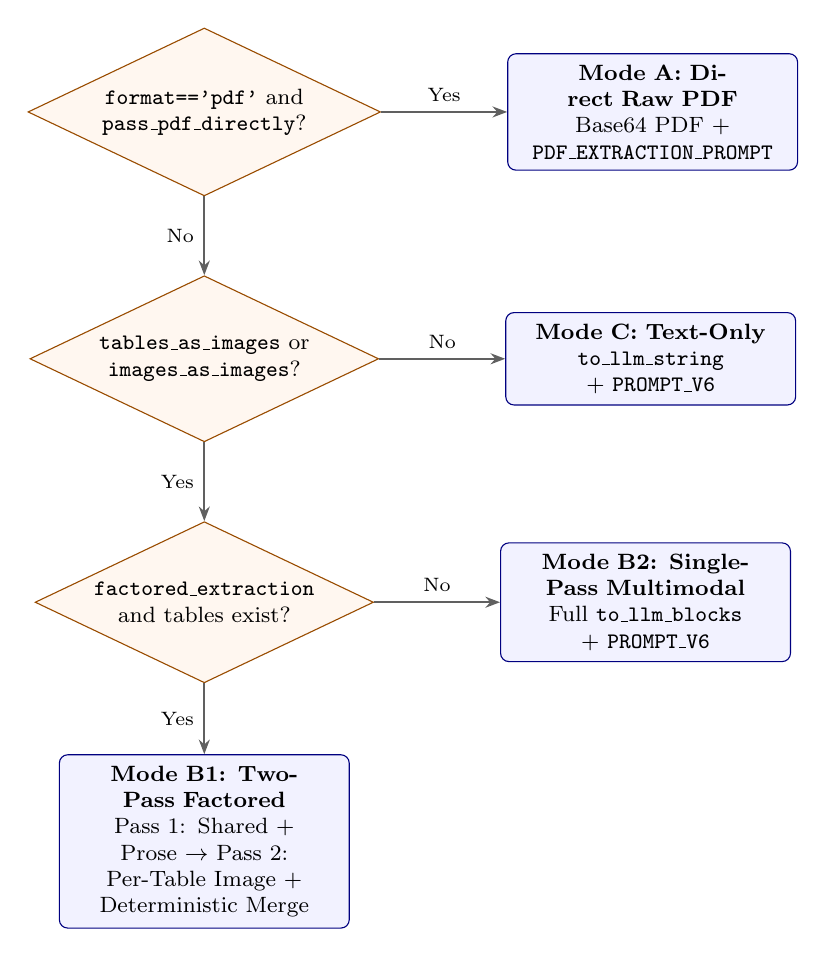
\begin{tikzpicture}[
    node distance=0.8cm and 1.2cm,
    decision/.style={diamond, aspect=2.1, draw=orange!60!black, fill=orange!6, text width=2.8cm, align=center, font=\footnotesize, inner sep=2pt},
    mode/.style={rectangle, rounded corners=3pt, draw=blue!50!black, fill=blue!5, text width=3.4cm, align=center, font=\footnotesize, minimum height=0.95cm, inner sep=4pt},
    arrow/.style={-{Stealth[scale=0.8]}, thick, draw=gray!75!black}
]
    \node[decision] (c1) {\texttt{format=='pdf'} and \texttt{pass\_pdf\_directly}?};
    \node[mode, right=1.6cm of c1] (mA) {\textbf{Mode A: Direct Raw PDF}\\Base64 PDF + \texttt{PDF\_EXTRACTION\_PROMPT}};

    \node[decision, below=1.0cm of c1] (c2) {\texttt{tables\_as\_images} or \texttt{images\_as\_images}?};
    \node[mode, right=1.6cm of c2] (mC) {\textbf{Mode C: Text-Only}\\ \texttt{to\_llm\_string} + \texttt{PROMPT\_V6}};

    \node[decision, below=1.0cm of c2] (c3) {\texttt{factored\_extraction} and tables exist?};
    \node[mode, right=1.6cm of c3] (mB2) {\textbf{Mode B2: Single-Pass Multimodal}\\Full \texttt{to\_llm\_blocks} + \texttt{PROMPT\_V6}};
    \node[mode, below=0.9cm of c3] (mB1) {\textbf{Mode B1: Two-Pass Factored}\\Pass 1: Shared + Prose $\rightarrow$ Pass 2: Per-Table Image + Deterministic Merge};

    \draw[arrow] (c1) -- node[above, font=\scriptsize] {Yes} (mA);
    \draw[arrow] (c1) -- node[left, font=\scriptsize] {No} (c2);
    \draw[arrow] (c2) -- node[left, font=\scriptsize] {Yes} (c3);
    \draw[arrow] (c2) -- node[above, font=\scriptsize] {No} (mC);
    \draw[arrow] (c3) -- node[above, font=\scriptsize] {No} (mB2);
    \draw[arrow] (c3) -- node[left, font=\scriptsize] {Yes} (mB1);
\end{tikzpicture}
\caption{Decision tree routing papers across the four LLM extraction pathways.}
\label{fig:extraction_routing}
\end{figure}

\begin{enumerate}
    \item \textbf{Mode A --- Direct Raw PDF (\texttt{pass\_pdf\_directly=True}):} Passes the raw base64-encoded PDF directly to a multimodal model alongside \texttt{PDF\_EXTRACTION\_SYSTEM\_PROMPT}. This avoids any GROBID parsing loss and yields high matrix unrolling recall, though without bracketed \texttt{Node} IDs for automated citation grounding.
    \item \textbf{Mode B1 --- Two-Pass Factored Extraction (default when visual blocks are enabled):} Designed to prevent LLMs from truncating large screening tables or omitting paper-wide defaults:
    \begin{itemize}
        \item \emph{Pass 1 (Paper-Wide Shared Conditions \& Prose):} Receives \texttt{prose\_text} (narrative text plus table/figure anchors) and extracts \texttt{SharedExperimentalConditions} (e.g., global temperature, buffer, detection methods, preparation protocol, and their \texttt{evidence\_span} tags) plus \texttt{prose\_entries} not covered by tables.
        \item \emph{Pass 2 (Per-Table Image Extraction):} Issues one independent multimodal call per cropped table image, conditioned on the Pass~1 shared summary and table caption, returning compact \texttt{TableExtractionResult} rows and tested condition cells.
        \item \emph{Deterministic Merge:} \texttt{merge\_table\_result\_with\_shared()} unrolls every $(\text{row}, \text{cell})$ pair into a full \texttt{PeptideLLMEntry} using strict precedence: $\text{cell} \rightarrow \text{row} \rightarrow \text{table\_defaults} \rightarrow \text{shared\_conditions}$, automatically populating \texttt{EvidenceSpan} with \texttt{[table\_id]} or the inherited Pass~1 prose tag.
    \end{itemize}
    \item \textbf{Mode B2 --- Single-Pass Multimodal:} Passes the complete \texttt{to\_llm\_blocks()} payload (interleaved or appendix) in a single call using \texttt{EXTRACTION\_SYSTEM\_PROMPT\_V6}.
    \item \textbf{Mode C --- Text-Only Citation-Grounded:} Passes \texttt{to\_llm\_string()} from JATS~XML or GROBID TEI~XML with \texttt{EXTRACTION\_SYSTEM\_PROMPT\_V6}.
\end{enumerate}

\subsection{Post-Extraction Normalization}
\texttt{peptide\_llm\_entry\_to\_peptide\_entry()} converts each \texttt{PeptideLLMEntry} into a database \texttt{PeptideEntry}: it enforces uppercase 1-letter IUPAC sequences, computes \texttt{length}, formats \texttt{volume\_ratio} lists (e.g., \texttt{[5, 95]} $\rightarrow$ \texttt{"5/95"}), joins \texttt{detection\_method} lists, serializes \texttt{evidence\_span} to JSON, and records \texttt{ExtractionMode.LLM} with the active \texttt{run\_identifier}.

\section{Evaluation and Empirical Results}
\label{sec:evaluation}

We evaluate \texttt{peptide\_extractor} using two complementary frameworks: (1) reference-free completeness and citation-grounding verification for unlabeled corpus-scale runs, and (2) normalized precision/recall/F1 benchmarking against manually curated golden entries.

\subsection{Reference-Free Grounding and Completeness}
For any extracted \texttt{PeptideEntry} and its source full text, \texttt{evaluate\_extraction()} (\texttt{evaluation.py}) computes:
\begin{itemize}
    \item \textbf{Completeness Rate:} Fraction of non-null fields out of 16 standard fields (or 17 when \texttt{peptide\_conjugate\_mixture} is \texttt{conjugate} or \texttt{mixture}, requiring \texttt{conjugate\_partner}).
    \item \textbf{Groundness Rate:} Fraction of checkable non-null fields verified against the source document:
    \begin{enumerate}
        \item \emph{Citation-Grounded Fields:} The 12 \texttt{EvidenceSpan} fields are resolved to their cited \texttt{Node} text via \texttt{get\_node\_by\_id()} and verified by an LLM judge (\texttt{deepseek-r1:8b} via Ollama).
        \item \emph{Verbatim Protocol:} \texttt{preparation\_protocol} is checked via exact substring match or \texttt{rapidfuzz} partial ratio $\ge 90.0$.
        \item \emph{Detection Methods:} Individual comma-separated techniques are matched against the full text (grounded if $\ge 80\%$ of listed methods match with partial ratio $\ge 90.0$).
    \end{enumerate}
\end{itemize}

\Cref{fig:eval_boxplots} and \Cref{fig:corpus_stats} show corpus-level evaluation distributions, column completion rates, peptide length distributions, and per-paper extraction counts generated by the visualization framework.

\begin{figure}[htbp]
\centering
\begin{subfigure}[b]{0.48\textwidth}
    \centering
    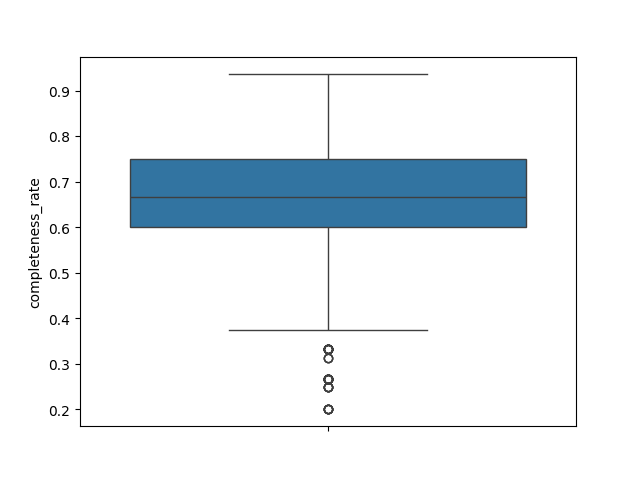
\includegraphics[width=\textwidth]{completeness_boxplot.png}
    \caption{Field completeness rate distribution}
    \label{fig:comp_box}
\end{subfigure}
\hfill
\begin{subfigure}[b]{0.48\textwidth}
    \centering
    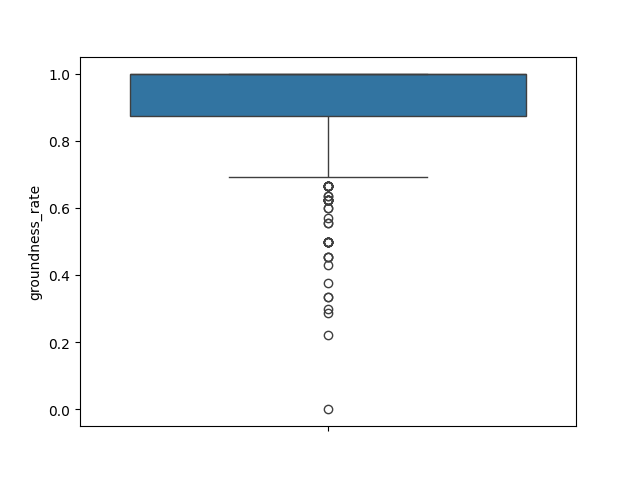
\includegraphics[width=\textwidth]{groundness_boxplot.png}
    \caption{Citation groundness rate distribution}
    \label{fig:ground_box}
\end{subfigure}
\caption{Reference-free evaluation distributions across extracted \texttt{PeptideEntry} records.}
\label{fig:eval_boxplots}
\end{figure}

\begin{figure}[htbp]
\centering
\begin{subfigure}[b]{0.48\textwidth}
    \centering
    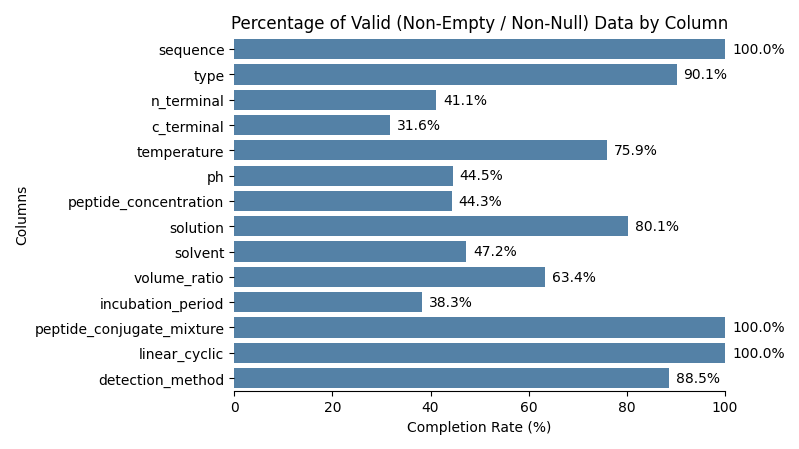
\includegraphics[width=\textwidth]{column_completion_final.png}
    \caption{Per-column completion rates}
    \label{fig:col_comp}
\end{subfigure}
\hfill
\begin{subfigure}[b]{0.48\textwidth}
    \centering
    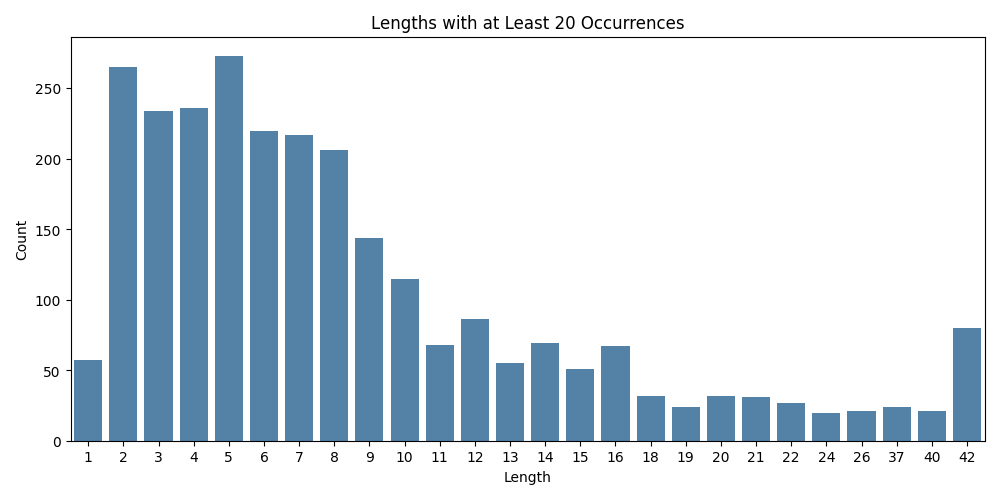
\includegraphics[width=\textwidth]{lengths_updated.png}
    \caption{Extracted peptide length distribution}
    \label{fig:len_dist}
\end{subfigure}
\caption{Extracted dataset characteristics across processed publications.}
\label{fig:corpus_stats}
\end{figure}

\subsection{Golden Dataset Benchmarking}
\texttt{benchmark\_run\_against\_golden()} (\texttt{golden\_benchmark.py}) compares LLM runs against \texttt{ExtractionMode.MANUAL} (\texttt{run\_identifier=0}) after canonicalizing terminal caps (\texttt{Ac} $\rightarrow$ \texttt{acetylation}, \texttt{NH2} $\rightarrow$ \texttt{amidation}), solvent tokens (\texttt{HFIP}/\texttt{HFP} $\rightarrow$ \texttt{hfp}), volume ratios, and numeric tolerances ($\pm 1.5\,^\circ\text{C}$ temperature, $\pm 0.2$ pH, $\pm 10\%$ relative concentration and incubation period). Entries are grouped by $(\text{pmid}, \text{sequence})$ and matched via greedy bipartite matching.

\Cref{tab:dev_benchmark} summarizes iterative progression across six runs on the 10-paper development slice (\texttt{DEV\_BENCHMARK\_PMIDS}: 56 manual sequences, 530 condition rows: 253 assembling, 277 non-assembling).

\begin{table}[htbp]
\centering
\caption{Development benchmark results across 10 multi-table golden papers (56 sequences, 530 condition rows).}
\label{tab:dev_benchmark}
\small
\begin{tabular}{@{}llcccccc@{}}
\toprule
\textbf{Run} & \textbf{Configuration} & \textbf{Seq R} & \textbf{Seq P} & \textbf{Seq F1} & \textbf{Rows} & \textbf{Matched} & \textbf{Cond P} \\
\midrule
Run 1 & Baseline (text, V4) & 28.6\% & 69.6\% & 40.5\% & 24 & 17 & 70.8\% \\
Run 2 & Multi-entry prompt (V5) & 28.6\% & 59.3\% & 38.6\% & 30 & 19 & 63.3\% \\
Run 3 & Mode A: Direct raw PDF & 91.1\% & 89.5\% & 90.3\% & \textbf{527} & \textbf{371} & 70.4\% \\
Run 4 & Mode C: PDF $\rightarrow$ text (V6) & 33.9\% & 82.6\% & 48.1\% & 90 & 67 & \textbf{74.4\%} \\
Run 5 & Mode B2: Table images (1-pass) & \textbf{92.9\%} & \textbf{91.2\%} & \textbf{92.0\%} & 359 & 258 & 71.9\% \\
Run 6 & Mode B1: Table images (2-pass) & 89.3\% & 83.3\% & 86.2\% & 444 & 302 & 68.0\% \\
\bottomrule
\end{tabular}
\end{table}

\subsection{Key Empirical Findings}
\begin{enumerate}
    \item \textbf{Visual Table Access is Critical:} Text-only GROBID conversion (Run~4) recovered only $33.9\%$ of sequences and $67/530$ condition rows ($12.6\%$). Passing cropped table images (Run~5) boosted sequence F1 to $92.0\%$ ($52/56$ sequences), while direct raw PDF (Run~3) achieved $90.3\%$ sequence F1 and matched $371/530$ condition rows ($70.0\%$: $57.3\%$ assembling recall, $81.6\%$ non-assembling recall).
    \item \textbf{Two-Pass Factoring Recovers Paper-Wide Defaults:} Single-pass table-image extraction (Run~5) achieved high sequence F1 ($92.0\%$) but frequently omitted paper-wide defaults under high row-count output---recovering temperature on only $40/258$ rows and incubation period on $23/254$ rows. Adding Pass~1 shared-condition extraction and deterministic merging (Run~6) increased matched rows from $258$ to $302$ ($+17\%$), restoring temperature coverage to $301/302$ ($99.7\%$ normalized accuracy) and incubation period coverage to $268/298$ ($92.2\%$ accuracy).
    \item \textbf{Remaining Field Normalization Gaps:} Across visual runs (Runs~3, 5, 6), normalized accuracy on \texttt{c\_terminal} ($4.0\%$--$24.3\%$) and \texttt{detection\_method} ($6.6\%$--$11.0\%$) lags behind \texttt{type} ($77.7\%$--$94.2\%$), \texttt{n\_terminal} ($91.4\%$--$96.8\%$), and \texttt{linear\_cyclic} ($93.0\%$--$97.7\%$), primarily due to differing conventions for amidated/free C-termini and per-method vs.\ per-experiment entry splitting in the golden dataset.
\end{enumerate}

\section{Conclusion and Future Work}
\label{sec:conclusion}

We have designed and implemented \texttt{peptide\_extractor}, an end-to-end automated curation pipeline for 4--20mer peptide self-assembly literature. By combining high-recall local abstract screening (saving $42.7\%$ of full-text processing across $\sim$50k papers), a unified JATS/TEI/PDF \texttt{Node} tree with PyMuPDF table cropping, and two-pass factored multimodal extraction, the system bridges the gap between unstructured scientific publications and auditable, schema-constrained relational records.

\subsection{Future Directions}
Several concrete avenues remain for improving extraction fidelity and coverage:
\begin{itemize}
    \item \textbf{Full 71-Paper Golden Evaluation:} Scale the Run~5/Run~6 multimodal and two-pass configurations from the 10-paper development slice to all 71 acquired SAPdb/PeptideMiner golden publications, and extend benchmarking to CPAD~2.0 and Cross-Beta~DB subsets.
    \item \textbf{Terminal and Method Harmonization:} Refine prompt instructions and canonicalization rules for \texttt{c\_terminal} notations (e.g., implicit free acid vs.\ \texttt{-NH2} amidation) and align \texttt{detection\_method} aggregation between golden entries and LLM outputs.
    \item \textbf{Hybrid Grounded Table-Image + Appendix Layout:} Evaluate \texttt{layout="appendix"} in \texttt{to\_llm\_blocks()} and enrich Pass~2 table prompts with cross-referenced footnote resolution so both high row recall and full \texttt{EvidenceSpan} auditability are preserved simultaneously.
    \item \textbf{Europe PMC Integration:} Complete \texttt{EuropePMCProvider} to expand open-access JATS~XML coverage and reduce reliance on PDF-to-TEI conversion.
\end{itemize}


\bibliographystyle{plainnat}
\bibliography{references}

\end{document}
